\documentclass[sigconf]{acmart}

\usepackage{booktabs} % For formal tables


% Copyright
%\setcopyright{none}
%\setcopyright{acmcopyright}
%\setcopyright{acmlicensed}
\setcopyright{rightsretained}
%\setcopyright{usgov}
%\setcopyright{usgovmixed}
%\setcopyright{cagov}
%\setcopyright{cagovmixed}

%Conference
\acmConference[Conference Name 2017]{ACM Short Name}{Month}{Location City, State, Country} 
\acmYear{2017}
\copyrightyear{2017}


\begin{document}
\newcommand\todo[1]{\textcolor{red}{#1}}

\title{Path Cost Analysis for Side Channel Detection}


\begin{abstract}
Side channels have been increasingly demonstrated as a practical threat to the confidentiality of private user information. Being able to statically detect these kinds of vulnerabilities is a key challenge in current computer security research. We introduce a new technique, path cost analysis (PCA), for the detection of side channels. Path cost analysis assigns a symbolic cost expression to every node and every back edge of a method's control flow graph. This cost expression gives an over-approximation for all possible observable values at that node or after traversing that cycle. Queries to a satisfiability solver on the maximum distance between specific pairs of nodes allow us to detect the presence of imbalanced paths through the control flow graph. When combined with taint analysis, we are able to answer the following question -- do there exist a pair of paths in the method's control flow graph, differing only on branch conditions influenced by the secret, which differ in observable value by more than some given threshold. In fact, we are able to specifically state what sets of secret-sensitive conditional statements introduce a side channel detectable given some noise parameter. We extend this approach to an interprocedural analysis, resulting in a sound over-approximation of the number of true side channels in the program. Greater precision can be obtained by combining our method with predicate abstraction or symbolic execution to determine whether a given path through the control flow graph is feasible. We propose evaluating our method on a set of sizeable java server-client applications. 
\end{abstract}

\keywords{Computer security, side channel analysis, static analysis}


\maketitle
\section{Introduction}

Modern software systems frequently store and manipulate personal data, such as location, credit card information or medical history.  Guaranteeing the confidentiality of such private data is necessary to protect the users of these systems.  To this end, the development of software systems is guided by the dictate that a program that manipulates private data should not reveal that data.  Many practices, such as the encryption of packages over a network, aim to protect the confidentiality of private data by ensuring that an observer is unable to parse any meaningful output from the system. Under these protections, the system's main channel, the content of the network packets, does not leak information about the private data. However, serious security vulnerabilities are still possible. 

A class of information leaks, called side-channel attacks use non-functional properties of the program's output to obtain information about private data.  Potential side channels include execution time, memory usage, size and timings of an encrypted series of packets, electromagnetic radiation and power consumption. For example, the timing and packet sizes of encrypted web trafic can leak information about what page a user has loaded. Side channels are properties of the implementation of the algorithm, not the algorithm itself. An algorithm may be secure but some aspect of its implementation, such as an optimization, can introduce a side channel that allows an observer to gain knowledge about protected data.  

Though side channel vulnerabilities have been know for many years, they are still often neglected by developers of web applications and other software services. They are commonly thought of as impratical despite a growing number of demonstrations of realistic side channel attacks that result in a critical security vulnerability \cite{timingpractical, cachepractical, ASLRtiming}. Because of this, programmers are often unaware of the potential side channels they may be introducing to a system, especially through attempts to optimize functions that manipulate secret input. To protect sensitive user data, scalable analysis tools devoted to the detection of side channel vulnerabilities are needed. We propose a static, scalable tool based on a method's control flow graph aimed at providing a sound over-approximation of the method's side channel vulnerabilities.  Our research aims to address the following questions:

\begin{itemize}
\item[] \textbf{RQ1.} Assume we are given a set of secret variables, a type of side channel, and a method's control flow graph. Can we detect the set of branch conditions responsible for potential side channels of the given type in the method and generate a pair of witness paths in the control flow graph for each? Witness paths are paths in the control flow graph differing only on the detected branch conditions whose observable output under the given side channel differs by more than some user defined threshold. 
\item[] \textbf{RQ2.} Can we extend this intraprocedural approach to an interprocedural one? 
\item[] \textbf{RQ3.} Can we iteratively refine the detected side channels by using predicate abstraction or a symbolic execution engine to detect when one of the witness paths is infeasible?
\item[] \textbf{RQ4.} How will our technique perform on large Java programs?
\end{itemize}

Our method is motivated by the observation that sizeable class of side channels occur when the value of private data results in multiple distinct control flow paths with characteristic observables. For example, the execution time of some implementations of the modular exponentiation function used RSA encryption take time proportional to the Hamming weight of the exponent. This is due to a branch condition repeated on each bit of the exponent which leads to additional computation whenever that bit is set to 1. Our hypothesis is that it is possible to detect the presence of these side channels from a method's control flow graph. We understand that not all side channels can be characterized by the above, such as those caused by low level issues like cache behavior \cite{cache}, but we still expect our method to be valuable in detecting a large class of side channels. Our expected contributions include a scalable static analysis tool to perform this detection and a iterative method to determine whether the detected side channels are actually exploitable in the program.
\section{Approach}

\textbf{Cost Model.} In general, we consider any program as a function of some input, some of which may be marked as private or secret. Any run of the function returns an observable value which represents the side channel measurements of that execution of function. 

Given a type of side channel, we can develop a cost model to approximate the output of that channel along a control flow path. For a given instruction, a cost model returns an expression for the observable of the considered channel. For example, a cost model for timing side channels might return the number of bytecode instructions, which can be used a proxy for execution time. These cost models provide static approximations of the observables that can be determined without running the program under test. Note that two executions of the same program with the same input might produce different observables --- for example, the execution time may be slightly different --- but the cost associated with their path through the control flow graph under the given cost model will remain the same.



\textbf{Path Cost Analysis.} The control flow graph of a program is a representation of all paths that might be traversed through a program during its execution. It is defined as a directed graph $G = (V, E)$ where the set of vertices $V$ are basic blocks and the set of edges $E$ represent jumps in the control flow. Path cost analysis is a technique we introduce to generate a symbolic expression for each node and back edge of the control flow graph which gives an over-approximation on the set of possible observable values at that node or for that cycle. Pairs of these symbolic cost expressions will be compared in order to detect paths in the control flow graphs that are imbalanced with respect to the given cost model. 


 %Our goal is to efficiently search the control flow graph for paths that are imbalanced with respect to our given cost model. Such an imbalance in the control flow graph marks a potential side channel in the method. To detect imbalanced paths, we introduce a method to annotate each node of the control flow graph with an expression that gives all potential cost values at the node, given a certain starting point. 
We do not analyze the entire control flow graph at once. Instead we perform an iterative analysis, first annotating smaller subgraphs and then combining the results to detect imbalance across these subgraphs. Our subgraphs are defined by the nesting structure of cycles in the control flow graph. If the control flow graph contains cycles, we annotate them first. Annotation of any cycle begins by recursively annotating its nested cycles. The base cases are cycles that contain no other cycles. To annotate a such a cycle, first remove the back edge, making an acyclic subgraph. It is now annotated as any other acyclic subgraph of the program. 

\textit{Annotation of Acyclic Graph:} To annotate an acyclic subgraph, we consider its nodes in topological order. The cost expression, $c_n$ of a node, $n$, is determined from the cost expressions of $n$'s immediate predecessors. Since $n$ represents a basic block of the method, let $|n|$ be the cost of this basic block under the given cost model (i.e. the number of bytecode instructions in $n$).  If $n$ has no predecessors, then $c_n$ is simply $|n|$.  If $n$ has one immediate predecessor, then its cost expression is the addition of $|n|$ and the cost expression of $n$'s immediate predecessor. If $n$ has two or more immediate predecessors, then two or more branches are merged at $n$. We will analyze the merging of each pair of branches individually. To do this, we will insert an additional node into the control flow graph for each additional merge in order of the most recently branched. These additional nodes will each have two incoming edges as will the original $n$. The cost expression for a node with two immediate predecessors is the addition of $|n|$ to $b \cdot c_{n-1} + (1 - b) \cdot c_{n-2}$, where nodes $n-1$ and $n-2$ are the two immediate predecessors of $n$ and $b$ is a fresh boolean variable. In this way, each branch condition is associated with a boolean variable, which represents whether the left of right branch was taken. See Fig~\ref{fig:merge} for the annotation of an acyclic subgraph with three paths merging at one node. The green node was added to the graph in order to merge the more recent left branch before the right. 

\begin{figure}
  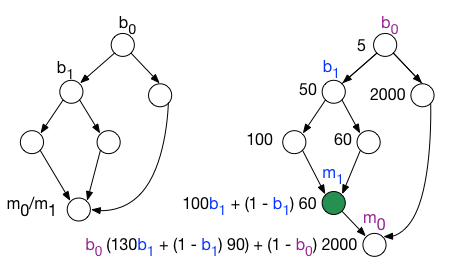
\includegraphics[scale=.5]{merge_paths.png}
  \caption{Left: original control flow graph. Right: annotated control flow graph.}
  \label{fig:merge}
\end{figure}

\vspace*{-0.1in} 


The only operation needed to generate the cost expression for a node in an acyclic graph is the addition of an integer to a cost expression. All possible cost expressions in an acyclic graph are given by:

$$Expr \rightarrow \begin{cases} Int  \\ b \cdot Expr_{0} + (1 - b) \cdot Expr_{1} \end{cases}$$

where b is a boolean variable, and $Expr_0$ and $Expr_1$ are the two possible cost expressions based on which branch to the most recent merge was taken. Addition by an integer is defined in each case as 

 $$Expr + Int \rightarrow \begin{cases} Int + Int \\ b \cdot (Expr_0 + Int) + (1 - b) \cdot (Expr_1 + Int) \end{cases}$$
  

%Since every node can only have up to two incoming edges and since the nodes of any non-cyclic graph can be annotated so that all predecessors of a node are annotated before that node, the above details a complete method for annotating the nodes of a non-cyclic subgraph.

\textit{Annotation of a Cyclic Subgraph.} The removed back edge is reintroduced and we derive its cost expression. We introduce a fresh integer variable $k$ denoting the number of times the cycle is taken. The cost expression of the cycle is now given by the product of the positive integer variable $k$ and the expression associated with the last node of the cycle. Multiplication by a integer variable is defined as 

 $$k \cdot Expr \rightarrow \begin{cases}  k \cdot Int \\ h \cdot Expr + (k - h) \cdot Expr \\\end{cases}$$
 
$h$ is a fresh variable which denotes the number of times out of the $k$ iterations of the cycle that a certain branch is taken. See Fig~\ref{fig:imb} for an example of how to annotate the back edge of a cycle.

\begin{figure}
  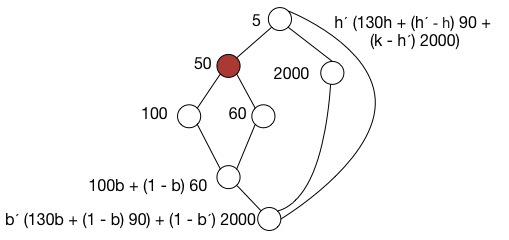
\includegraphics[scale=.5]{imbalance.png}
  \caption{Annotated control flow graph with a cycle. Red node is a branch on a secret variable.}
  \label{fig:imb}
\end{figure}

Finding the cost expressions for all nodes and back edges of a control flow graph can now be described as follows -- first recursively find the costs of all nested cycles, then treat each nested cycle as a single node for which $|n|$ is given by the cost of the cycle. This extends the set of possible cost expressions to include 

$$Expr \rightarrow \begin{cases} k \cdot Int  \\ h \cdot Expr_{0} + (k - h) \cdot Expr_{1} \end{cases}$$

and the rules for addition by an integer or multiplication by another loop variable are extended appropriately. 
 
\textbf{Imbalance Detection.} Given the annotated control flow graph, we compare select pairs of cost expressions to detect the presence of imbalanced control flow paths. These cost expressions are compared using a satisfiability solver such as z3 \cite{z3} or cvc4 \cite{cvc4} to determine whether there are satisfying solutions of their variables for which the distance between the two costs is higher than some user-provided threshold. There are three types of pairs of cost expressions to compare. 

1)\textit{ Output nodes.} Output nodes are any nodes in the control flow graph at which the observable may be measured when running the program. For example, any node where a packet is sent over the network is an instance of where an observable such as time or packet size could be collected. Not all output nodes need be compared with each other. To determine which output nodes to compare, we search the control flow graph to determine the set of \textit{output predecessors} for each output node. A node $p$ is an output predecessor of node $n$ if $p$ is either itself an output node or a node with no incoming edges and there is some path to $n$ including $p$ such that between some occurrence of $p$ and $n$, there is no other output node. Note that in the presence of loops, $n$ can be a predecessor of itself. Two non-identical output nodes are compared only in the case that intersection of their predecessor nodes is nonempty. An output node is compared with itself if there are two distinct paths to the output node with identical predecessors.  

2) \textit{ Secret Dependent Branch Conditions}  A branch condition is said to be dependent on a secret value if the value of any of its variables can be affected by the secret. For any branch condition in the control flow graph that depends on the secret value and does not form a back edge, we compare the cost expressions of the immediate predecessors of the node that merges the paths resultant from this branch. For any cycle in the control flow graph containing a conditional statement that depends on the secret value, we compare two copies of the cost expression of its back edge, each with its own set of fresh variables. 

% Likewise, for each back edge of the control flow graph, we consider the symbolic cost of the associated cycle and query the satisfiability solver to determine whether there are two distinct paths through the cycle such that the difference between the costs is greater than the threshold. 


%This result informs us as to whether there are two distinct paths in the control flow graph to the considered merge that are sufficiently imbalanced under the given cost model according to some threshold.

%This threshold can depend on the cost model and the expected noise of the system. For example, if the side channel is deterministic such the size of an output file, then the threshold might simply be zero. However, in the case where there is some system noise associated with the side channel, such as execution time, a higher threshold might be appropriate. 

%The number of nodes compared in the control flow graph is constant in the number of conditionals in the program. There is one additional set of nodes to be compared, which we refer to as output nodes. Output nodes are any nodes in the control flow graph at which the observable may be measured when running the program. For example, any node where a packet is sent over the network is an instance of where an observable such as time or packet size could be collected. Not all output nodes need be compared with each other. To determine which output nodes to compare, we search the control flow graph to determine the set of predecessors for each output node. A node $p$ is an predecessor of node $n$ if $p$ is either itself an output node or a node with no incoming edges and there is some path to $n$ including $p$ such that between some occurence of $p$ and $n$, there is no other output node. Note that in the presence of loops, $n$ can be a predecessor of itself. Two non-identical output nodes are compared only in the case that intersection of their predeccesor nodes is nonempty. An output node is compared with itself if there are two distinct paths to the output node with identical predecessors.  

%Regardless of what kind of nodes the query is on, the result is not only a boolean response as to the presence of imbalanced paths through the control flow graph but also a satisfying solution as to which branch conditions differ produce a pair of imbalanced paths. However, there might be many imbalanced paths that do not leak any information about the secret variables. This is because none of the differing branch conditions have any relation to the secret variables. In order to make our analysis more precise, we combine it with taint analysis to mark each branch condition in the control flow graph as dependent on a secret value or independent. A conditional is said to be dependent on a secret value if the value of any of its variables can be effected by the secret.

In all cases, the query to the satisfiability solver is constrained as follows. Both paths must agree on any variable whose associated branch condition does not depend on the secret value. The pair of witness paths returned by the satisfiability solver will be distinct paths in the control flow graph that differ on at least one branch condition that is dependent on the secret. Since the two paths are differentiable with respect to our cost model, this is exactly what it means for a side channel to be present. 

Consider the case in Fig~\ref{fig:imb} for a threshold of 100. The only branch statement is  that depends on the secret is $b_1$, the red node. To see if this branch statement alone induces a side channel, we compare the costs of the immediate predecessors of $m_1$, 100 and 60, to see that this side channel is not strong enough to be detected for the threshold. Since the branch at the first node of the graph, $b_0$ is not dependent on the secret we do not have to compare the two predecessors of its merge $m_0$. Finally, we consider the cost of the back edge. In this case, we set the maximum number of loop iterations to three and impose the constraint, $k \leq 3$. We compare two versions of the symbolic cost of the back edge, each with its own set of variables. Since neither the value of first branch nor the loop condition depends on the secret, the values of $h_0$ and $k$ must match. Only the value of $h_1$ may differ. In this case, we discover that $k = 3, h_0 = 3,h_1 = 3$ and $k = 3, h_0 = 3, h_1 = 0$ give two paths through the control flow graph, differing only on the branch condition at the node marked $b_1$, for which the difference in cost is greater than the given threshold. 
\section{Improvments}
\subsection{Extension to Interprocedural Analysis}
The approach above is an intraprocedural analysis performed on the control flow graph of a method. We will also try to extend this apporach to an interprodecural analysis. When no recursion is present in the program, we will create a in-lined control flow graph where function calls are replaced by the control flow graph of the called method. Each function call creates a new copy of its control flow graph, which adds calling context to the analysis. In the case of recursion -- we will explore two possible avenues. One is to bound the depth of recursion and use the same inlining method as above. The second is to create a back-edge in the control flow graph to represent the recursion. While this results in additional infeasible paths added to our analysis as the calling context is lost, all possible control flow paths will be present, preserving the soundness of our analysis. 

\subsection{Refinement}

While our method returns a sound over-approximation of side channels up to a user-specified strength in the source code, it is not precise. This stems from the fact that not all paths in the control flow graph are feasible, and hence a detected side channel may not be exploitable in the executable program. To help mitigate this problem, we will explore combining our analysis with predicate abstraction \cite{predicate}. Predicate abstraction allows us to define a set of predicates on program variables and keep track of the possible values of those predicates through transitions of a finite state machine. In our case, we will be using the conditions of the branch statements along our witness paths as the set of predicates. Predicate abstraction will allow us to determine if the values of the predicates along the considered path are unsatisfiable. Since predicate abstraction provides an overapproximation for the possible values of the predicates, we will still conclude that some unexploitable side channels are realizable; however, our hypothesis is that predicate absraction will still be beneficial in reducing the number of unrealizable side channels reported. 

A potential hurdle in effectively using predicate abstraction to reduce the number of paths is that there may not only be a single pair of witness paths for a side channel but rather a space of potential witness paths. We would need to check the feasibility of each of these paths which in the worst case could be an exponential number. We believe that our choice to independently analyze subgraphs of the control flow will help with exponential blow-up but it could remain a problem nevertherless. Additionally, since predicate abstraction provides an over-approximation, we cannot conclude that a side channel exists even when the considered paths are found to be not be unfeasible. The only conclusion we might be able to make is that a detected side channel is infeasible. 

Another potential way to determine if a side channel is exploitable is to use a method such as symbolic execution \cite{symbolic} to obtain the path condition that must be satisfied for the considered path to be feasible.  This would allow us to obtain an accurate answer as to whether a pair of witness paths are realizable. In this case, we would be able to positvely answer that a side channel in the program is detectable within the threshold. Again, there may be an exponential number of paths making this approach infeasible in the worst case. However, once we ascertain that one particular pair of witness paths are satisfiable, we have proven the existence of an exploitable side channel in the program and do not need to continue the analysis. This allows us to postively answer the question of side channel existence. 
\section{Evaluation}

We propose to evaluate our tool on a series of Java programs from the DARPA STAC program as well as a set of classic side channel vulnerabilites, such as CRIME \cite{crime} and simple string comparison. The DARPA STAC programs are sizeable, containing thousands of methods. Side channel vulnerabilities are either in timing or space, such as the sizes of encrypted packets. We plan to evaluate our method based on its ability to correctly locate side channel vulnerabilities in each of these programs. Our method will be considered successful if it is able to identify the branch conditions responsible for a side channel that leaks information about the provided secret value. Since our method is designed to be an over-approximation, we also plan to evaluate how useful predicate abstraction and symbolic execution are at reducing the number of false positives. 

%Since our method depends on a user defined threshold for the imbalance between paths, our test suite will also provide an means to evaluate the importance of this threshold. We plan to use this test suite to determine suitable values for both timing and space side channels. In the case of timing side channels, the threshold should be high enough so that the difference in time is observable even across a network. If the side channels in space are deterministic, then it may be the case that a threshold of zero is appropriate. \todo{probably to remove for space}
\section{Related Work}

There has been notable previous work on static analysis for side channel detection. One type of approach is that of by Pasareanu et al. \cite{smtmulti} and Bang et al. \cite{BAQ16}. They both use a combination of symbolic execution and model counting to determine the probability of a particular execution path and tools from information theory to determine the amount of leakage based on those probabilities. This kind of approach suffers due to its reliance on symbolic execution which does not scale to large applications. Our approach could be considered complimentary to theirs. Using PCA, we can reduce a complicated program to a potentially much smaller set of suspicious methods for which symbolic execution might be scalable. Work by Zhang et al. on Sidebuster \cite{sidebuster} details a static approach to detecting side channels in web applications. Their work involves taint analysis to determine whether a secret value has propagated to a conditional branching statement. If it has, the number of remote procedure calls in each branch are compared. If the number of calls differs, the site is marked as a potential side channel. Both this approach and ours are built on detecting differences in branches resultant from conditionals dependent on the secret value, but the symbolic cost expressions key to PCA make it a much more expressive method. Another static approach is presented by Antopolous et al. in their tool Blazer \cite{decomposition}. Their approach involves recursively partitioning the set of possible traces through the program such that all traces in a given partition take approximately the same amount of time. Other types of static analysis techniques are particular to specific types of side channels, such as CacheAudit \cite{cacheaudit}, or are type-based analyses \cite{fixbyconstant,hedin}.

%Previous work on side channel detection and quantification can be broken down into static and dynamic approaches. Dynamic approaches, such as presented by Chothia et al. in their tool LeakWatch \cite{leakwatch} estimate the amount on leakage in a given program through statistical analysis \cite{formalbounds, stats} done on the repeated trials of the program using independently drawn input samples. \todo{probably remove all dynamic stuff} Our work is more closely related to other static techqniues to detecting side channels. 
\bibliographystyle{ACM-Reference-Format}
\bibliography{biblio}

\end{document}
